\begin{lstlisting}[numbers=none]
package main

import (
    "fmt"
    "net/http"
    "strings"
    "log"
)

func sayhelloName(w http.ResponseWriter, r *http.Request) {
    r.ParseForm()  //オプションを解析します。
                   //デフォルトでは解析しません。
    fmt.Println(r.Form)
    //このデータはサーバのプリント情報に出力されます。
    fmt.Println("path", r.URL.Path)
    fmt.Println("scheme", r.URL.Scheme)
    fmt.Println(r.Form["url_long"])
    for k, v := range r.Form {
        fmt.Println("key:", k)
        fmt.Println("val:", strings.Join(v, ""))
    }
    fmt.Fprintf(w, "Hello astaxie!")
    //ここでwに入るものがクライアントに出力されます。
}

func main() {
    http.HandleFunc("/", sayhelloName)
    //アクセスのルーティングを設定します。
    err := http.ListenAndServe(":9090", nil)
    //監視するポートを設定します。
    if err != nil {
        log.Fatal("ListenAndServe: ", err)
    }
}
\end{lstlisting}

上のコードはbuildした後、web.exeを実行した際、9090ポートでhttpリンクリクエストを監視します。

ブラウザで\texttt{http:\/\//\/\//localhost:9090}を入力してください。

ブラウザでHello astaxie!と出力されたのが見えたかと思います。

アドレスを変えて試してみましょう:\texttt{http:\//\//localhost:9090\//?url\_long=111\&url\_long=222}

ブラウザで出力されたものは何でしょうか。サーバは何と出力していますか?

サーバで出力される情報は以下の通りです:

\begin{figure}[H]
  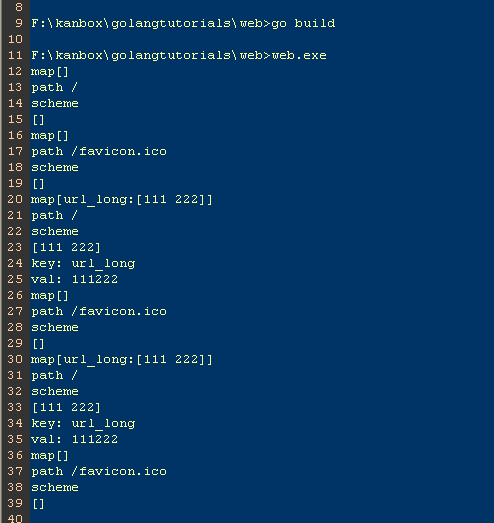
\includegraphics[width=14cm]{3.2.goweb.png}
   \label{図3.8}
   \caption{ユーザがWebにアクセスしてサーバが出力する情報}
\end{figure}

上のコードでWebサーバを書くためにはhttpパッケージの2つの関数を呼ぶだけで良いことがわかります。


\begin{quote}
もしあなたが以前PHPプログラマであれば。こう問うかもしれません。我々のnginx、apacheサーバは必要ないのですかと?なぜならこいつは直接tcpポートを監視しますので、nginxがやることをやってくれます。またsayhelloNameは実は我々が書いたロジック関数ですので、phpの中のコントローラ(controller)関数に近いものです。

もしあなたがPythonプログラマであったのなら、tornadoを聞いたことがあると思います。このコードはそれとよく似ていませんか?ええ、その通りです。GoはPythonのような動的な言語によく似た特性を持っています。Webアプリケーションを書くにはとても便利です。

もしあなたがRubyプログラマであったのなら、RORの/script/serverを起動したのと少し似ている事に気づいたかもしれません。
\end{quote}


Goを通じて簡単な数行のコードでwebサーバを立ち上げることができました。さらにこのWebサーバの内部ではマルチスレッドの特性をサポートしています。続く2つの節でGoが如何にWebのマルチスレッドを実現しているのか細かくご紹介します。
